\section{Spüre die Welt – Bedingte Anweisung und Verzweigung}

\subsection{Mal ein Labyrinth}

Wir brauchen ein Labyrinth als Barriere für unsere Hauptfigur. Wir erzeugen dazu ein weiteres Sprite, welches als Barriere dient.

\begin{itemize}
\item[1.] Klicke auf das \textit{Neues Objekt malen}-Icon.
\end{itemize}
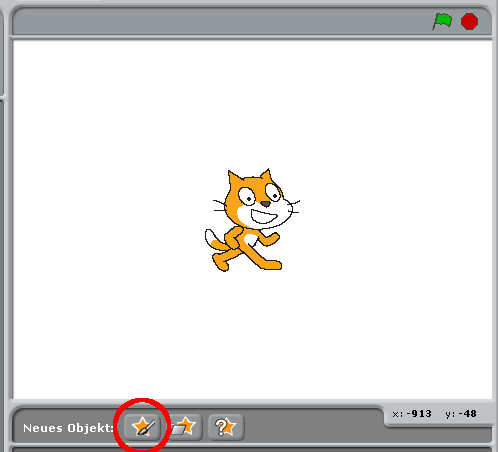
\includegraphics[width=0.6\textwidth]{images/aufgabe2_neues_objekt_malen.png}
\begin{itemize}
\item[2.] Benutze das Zoom-Tool um komplett herauszuzoomen. Klicke auf die Minus-Lupe.
\end{itemize}
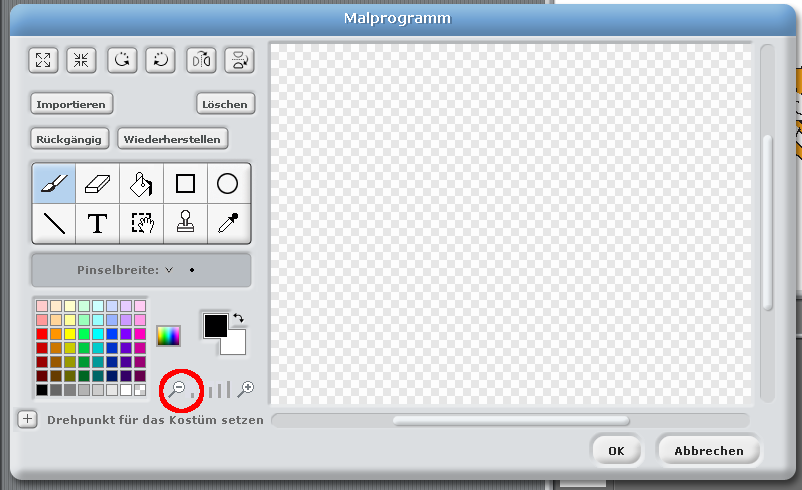
\includegraphics[width=0.6\textwidth]{images/aufgabe2_zoom.png}
\begin{itemize}
\item[3.] Klicke auf das Rechteck-Symbol und male eine Rechteck um die gesamte Bildfläche.
\end{itemize}
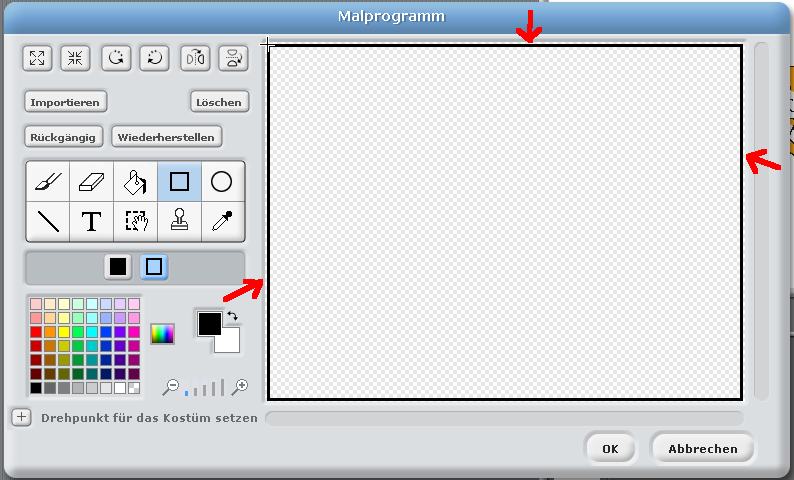
\includegraphics[width=0.6\textwidth]{images/aufgabe2_rechteck_gross.png}
\begin{itemize}
\item[4.] Benutze das Rechteck Tool mit ausgewähltem Füllmodus, um einige Hindernisse zu malen.
\end{itemize}
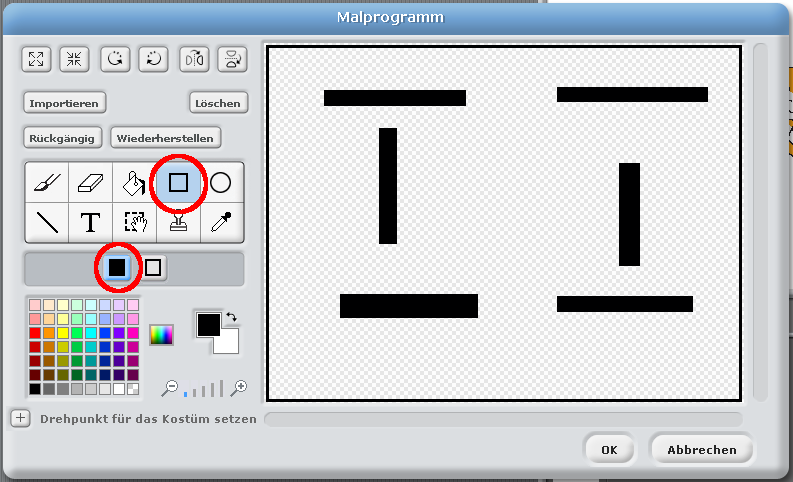
\includegraphics[width=0.6\textwidth]{images/aufgabe2_labyrinth.png}
\begin{itemize}
\item[5.] Klicke auf Ok, um deine Zeichnung abzuschließen.
\item[6.] Ändere den Namen des Sprites zu Labyrinth.
\end{itemize}

\subsection{Abprallen vom Hinderniss}
\begin{itemize}
\item[1.] Klicke auf deine Sprite-Figur.
\item[2.] Ziehe jetzt aus dem Steuerung-Panel, das \textit{Wenn grüne Flagge angeklickt} in das Skript-Panel.
\end{itemize}

\includegraphics[width=0.6\textwidth]{images/aufgabe2_automat0.png}
\begin{itemize}
\item[3.] Füge nun das \textit{wiederhole fortlaufend} hinzu.
\end{itemize}
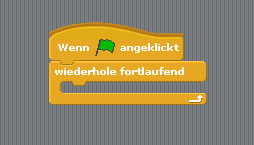
\includegraphics[width=0.6\textwidth]{images/aufgabe2_automat1.png}
\begin{itemize} 
\item[4.] Füge nun aus dem Bewegungs-Panel, \textit{gehe 10er Schritt} in die Lücke.
\end{itemize}
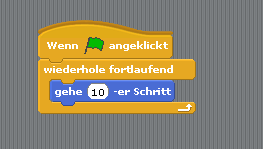
\includegraphics[width=0.6\textwidth]{images/aufgabe2_automat2.png}
\begin{itemize}
\item[5.] Hänge daran nun aus dem Steuerungs-Panel, die Kachel \textit{falls} hinzu.
\end{itemize}
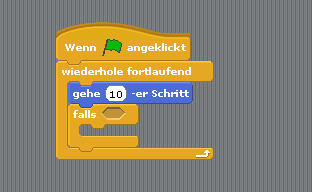
\includegraphics[width=0.6\textwidth]{images/aufgabe2_automat3.png}
\begin{itemize}
\item[6.] Wechsle nun in das Fühlen-Panel
\end{itemize}
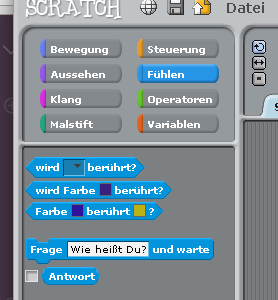
\includegraphics[width=0.6\textwidth]{images/aufgabe2_fuehlen.png}
\begin{itemize}
\item[7.] Wähle nun die \textit{wird berührt}-Kachel, ziehe es ins Skript-Panel in die Wabe der Falls-Kachel und wähle dort das Labyrinth. 
\end{itemize}
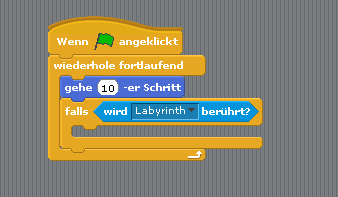
\includegraphics[width=0.6\textwidth]{images/aufgabe2_automat4.png}
\begin{itemize}
\item[8.] Anschließend wählst du aus dem Bewegungs-Panel \textit{drehe um 90 Grad} und \textit{gehe 10-er Schritte} und ziehst es in die Lücke unter \textit{falls}.
\end{itemize}
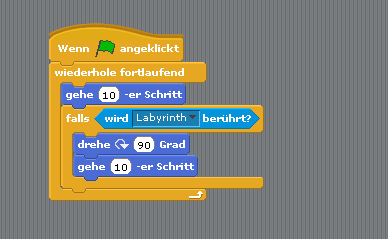
\includegraphics[width=0.6\textwidth]{images/aufgabe2_automat5.png}
\begin{itemize}
\item[9.] Teste dein Programm. Drücke auf die grüne Flagge und starte dein Programm. Beeinflusse die Richtung mit Hilfe der Pfeiltasten deiner Tastatur.
\end{itemize}
